\documentclass[11pt]{article}
\usepackage[a4paper,margin=1in]{geometry}
\usepackage{graphicx}
\usepackage{listings}
\usepackage{xcolor}
\usepackage{booktabs}
\usepackage{array}
\usepackage{hyperref}
\usepackage{parskip}
\hypersetup{colorlinks=true, linkcolor=black, urlcolor=blue}

\definecolor{codebg}{RGB}{245,245,245}
\lstdefinestyle{cstyle}{
  language=C,
  backgroundcolor=\color{codebg},
  basicstyle=\ttfamily\footnotesize,
  keywordstyle=\color{blue}\bfseries,
  commentstyle=\color{gray}\itshape,
  stringstyle=\color{teal},
  numbers=left,
  numberstyle=\tiny\color{gray},
  stepnumber=1,
  breaklines=true,
  frame=single,
  tabsize=2,
  showstringspaces=false
}
\lstdefinestyle{outstyle}{
  backgroundcolor=\color{codebg},
  basicstyle=\ttfamily\footnotesize,
  breaklines=true,
  frame=single,
  showstringspaces=false
}

\title{\vspace{-2cm}}
\date{}

\begin{document}
\begin{titlepage}
\centering
\vspace*{1cm}
{\large \textbf{Sri Sivasubramaniya Nadar College of Engineering}}\\
{\small (An Autonomous Institution, Affiliated to Anna University, Chennai)}\\
{\small Kalavakkam -- 603 110}\\[0.3cm]
{\small Department of Computer Science \& Engineering}\\[1.5cm]

\rule{\linewidth}{0.5mm}\\[0.4cm]
{\LARGE \textbf{Computer Networks Laboratory}}\\[0.3cm]
{\Large 1513 -- Computer Networks Lab}\\[0.4cm]
\rule{\linewidth}{0.5mm}\\[1.5cm]

{\huge \textbf{Assignment 2}}\\[0.4cm]
{\Large Multi-Client Chat Application using TCP and UDP Sockets}\\[2cm]

\begin{center}
\begin{tabular}{ll}
\textbf{Name:} & Simiyon Vinscent Samuel L \\[0.2cm]
\textbf{Register Number:} & 3122247001062 \\[0.2cm]
\textbf{Year / Semester:} & III Year / V Semester \\[0.2cm]
\textbf{Course:} & 1513 Computer Networks Lab \\[0.2cm]
\textbf{Date of Submission:} & 06 March 2026 \\[0.2cm]
\end{tabular}
\end{center}

\vfill
\end{titlepage}

\section*{1. Objective}
To design and implement client--server applications in C using socket programming that allow
students to retrieve academic information (stored in a CSV file \texttt{students.csv}) from a
server, using both TCP (connection-oriented) and UDP (connectionless) transport, and to compare
the two implementations based on connection setup, reliability, ordering, error recovery, and
communication overhead.

\begin{itemize}
  \item \textbf{TCP application:} retrieve the complete academic profile of a student given a Roll
  Number, with the server handling multiple clients concurrently using POSIX threads.
  \item \textbf{UDP application:} verify a student record (Roll Number and Name only) using a
  single connectionless datagram exchange.
\end{itemize}

\section*{2. Server Algorithm}
\subsection*{2.1 TCP Server}
\begin{enumerate}
  \item Create a TCP socket using \texttt{socket(AF\_INET, SOCK\_STREAM, 0)}.
  \item Set \texttt{SO\_REUSEADDR} and bind the socket to port 8080 using \texttt{bind()}.
  \item Call \texttt{listen()} to mark the socket as passive and wait for connections.
  \item In an infinite loop, \texttt{accept()} an incoming client connection.
  \item Spawn a new POSIX thread (\texttt{pthread\_create}) per client so multiple clients are
        served concurrently; detach the thread.
  \item Inside the thread: \texttt{recv()} the Roll Number, linearly search \texttt{students.csv}
        for a matching record.
  \item If found, format and \texttt{send()} the full record (Roll No, Name, Department, Semester,
        CGPA); otherwise send \texttt{"Student Record Not Found"}.
  \item Close the client socket and terminate the thread.
\end{enumerate}

\subsection*{2.2 UDP Server}
\begin{enumerate}
  \item Create a UDP socket using \texttt{socket(AF\_INET, SOCK\_DGRAM, 0)}.
  \item Bind the socket to port 8081 using \texttt{bind()}.
  \item In an infinite loop, block on \texttt{recvfrom()} to receive a Roll Number datagram
        together with the client's address.
  \item Search \texttt{students.csv} for the Roll Number.
  \item If found, build a short reply containing only Roll Number and Name; otherwise reply
        \texttt{"Student Record Not Found"}.
  \item Send the reply back to the client's address using \texttt{sendto()} (no connection state
        is kept).
\end{enumerate}

\section*{3. Client Algorithm}
\subsection*{3.1 TCP Client}
\begin{enumerate}
  \item Create a TCP socket and \texttt{connect()} to the server at \texttt{127.0.0.1:8080}.
  \item Prompt the user to enter a Roll Number and \texttt{send()} it to the server.
  \item Loop on \texttt{recv()} until the connection is closed, printing the received bytes.
  \item Close the socket.
\end{enumerate}

\subsection*{3.2 UDP Client}
\begin{enumerate}
  \item Create a UDP socket (no \texttt{connect()} required).
  \item Prompt the user for a Roll Number and \texttt{sendto()} it to \texttt{127.0.0.1:8081}.
  \item Block on \texttt{recvfrom()} to receive the server's reply.
  \item Display the reply and close the socket.
\end{enumerate}

\section*{4. Server Code}
\subsection*{4.1 tcp\_server.c}
\lstinputlisting[style=cstyle]{tcp_server.c}
\subsection*{4.2 udp\_server.c}
\lstinputlisting[style=cstyle]{udp_server.c}

\section*{5. Client Code}
\subsection*{5.1 tcp\_client.c}
\lstinputlisting[style=cstyle]{tcp_client.c}
\subsection*{5.2 udp\_client.c}
\lstinputlisting[style=cstyle]{udp_client.c}

\section*{6. Output / Test Cases}
Both servers were started in the background and the clients were run against Roll Numbers that
exist in \texttt{students.csv} (e.g.\ 101, 102) as well as one that does not (999), to test both
the success and \emph{record-not-found} paths.

\subsection*{6.1 Screenshots}
\begin{figure}[h!]
\centering
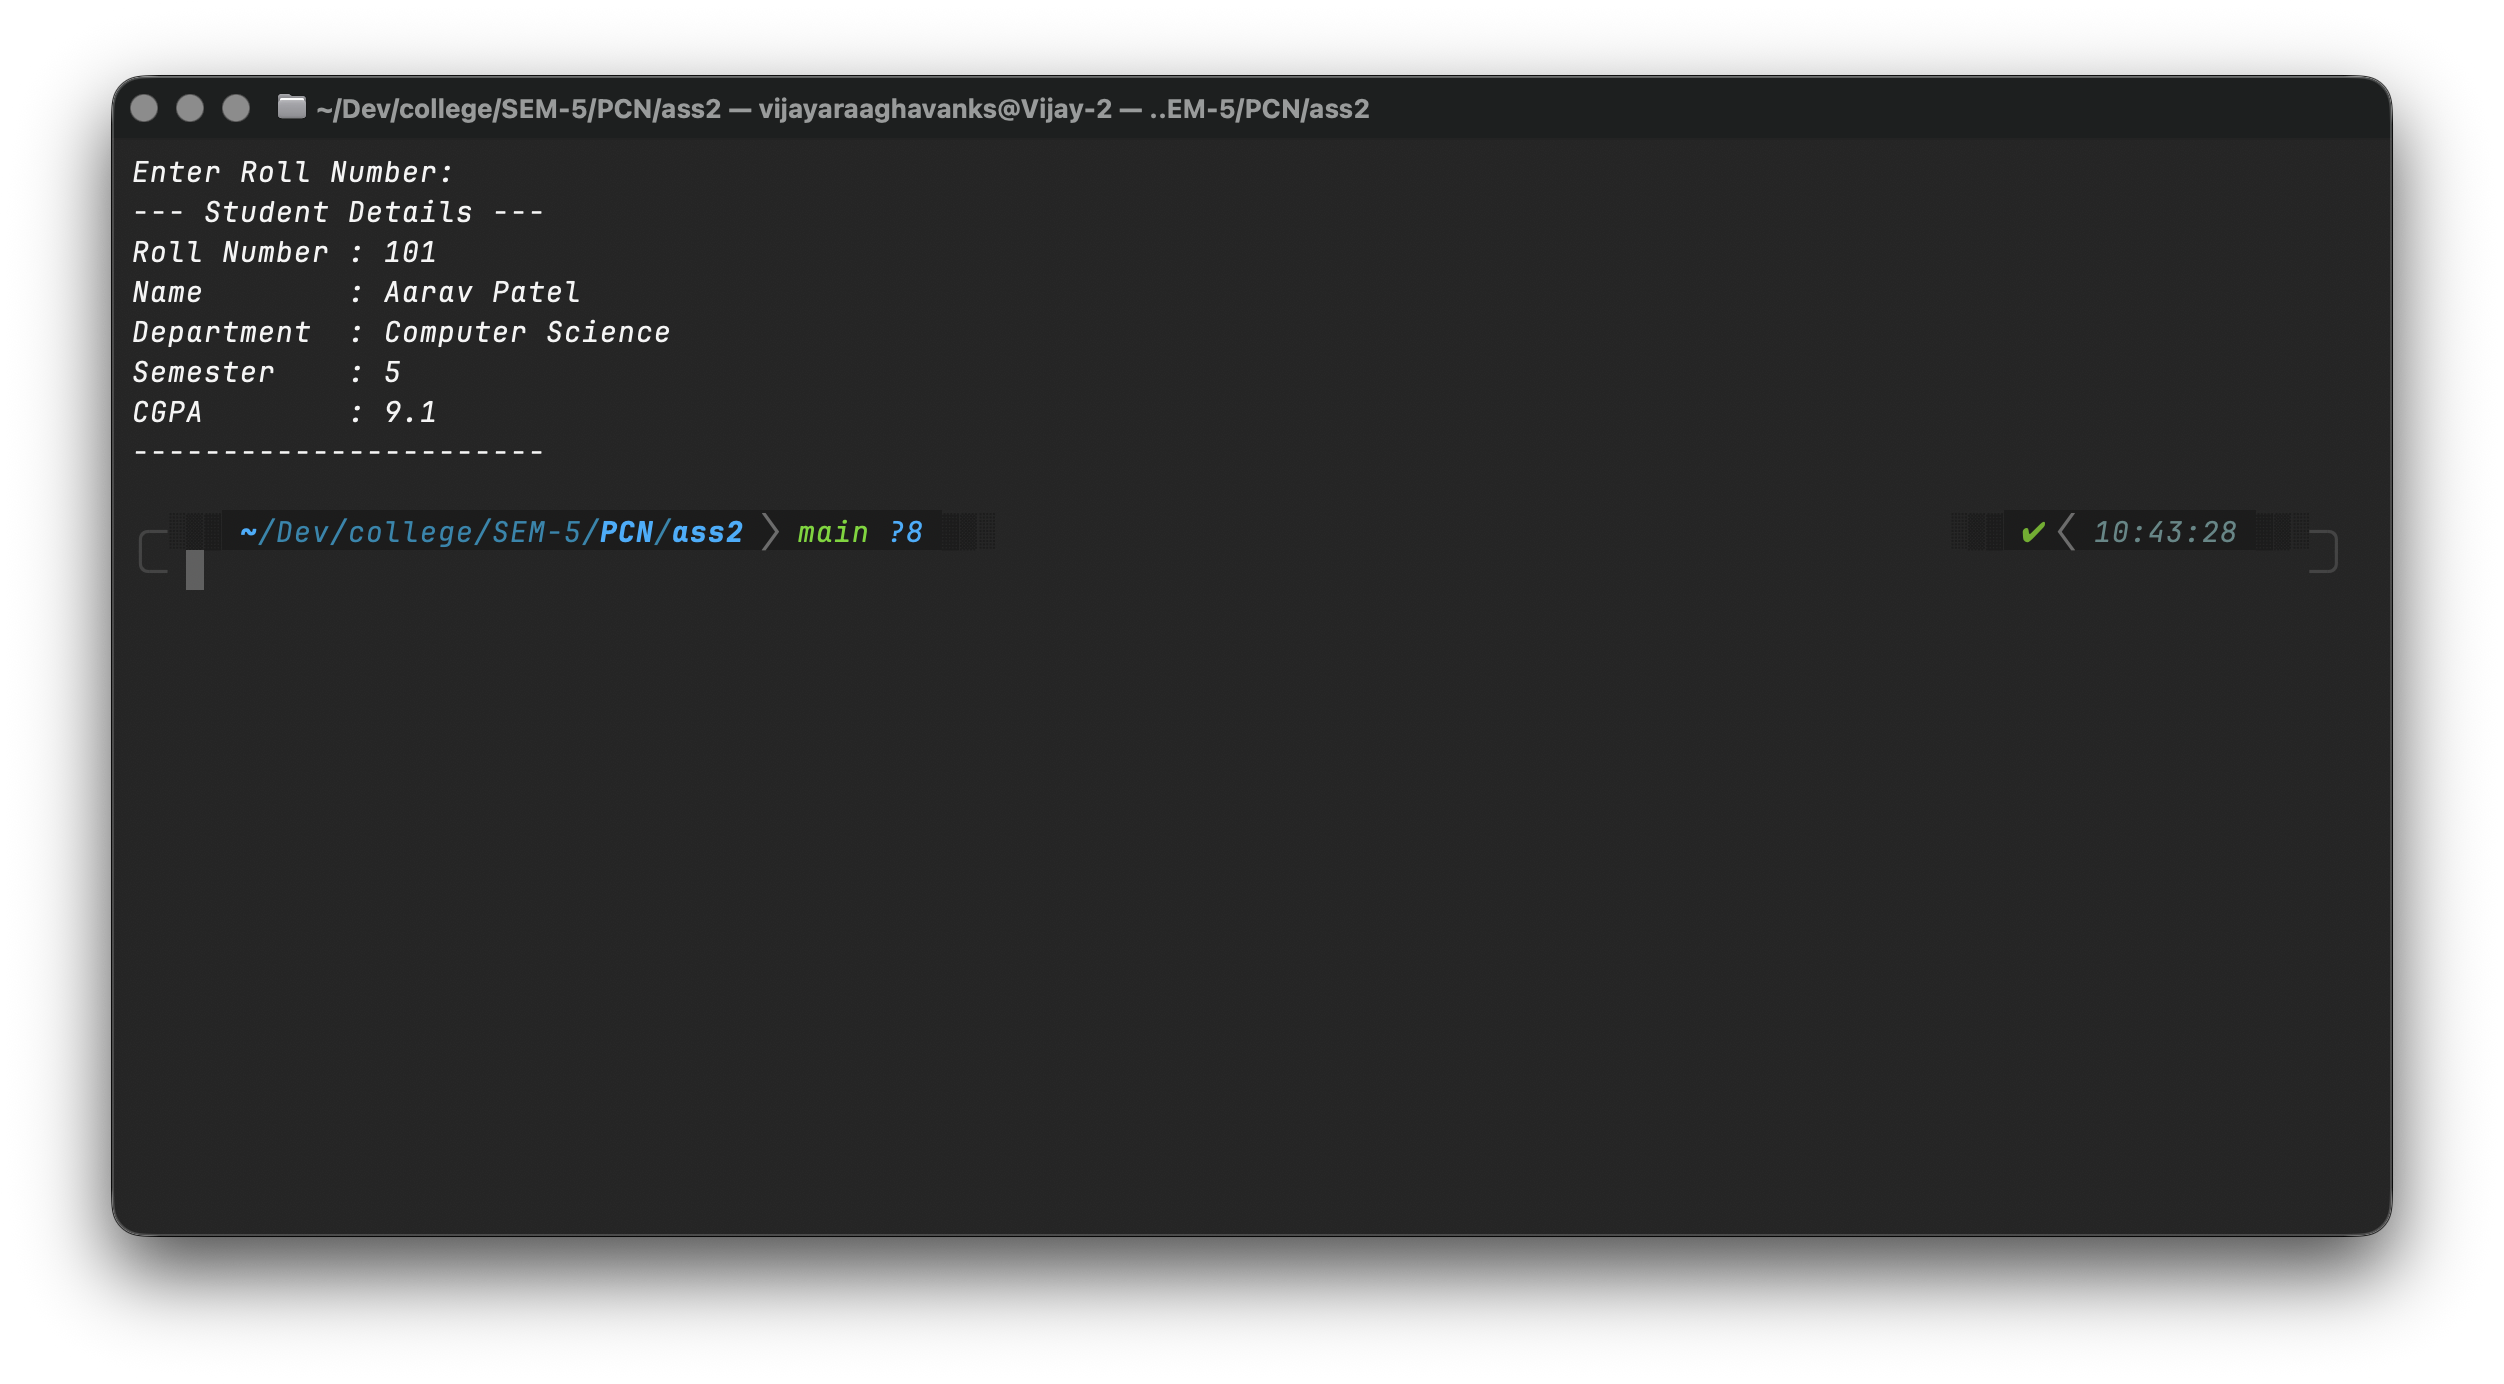
\includegraphics[width=0.62\linewidth]{screenshots/01_tcp_client_found.png}
\caption{TCP client -- record found (Roll Number 101)}
\end{figure}

\begin{figure}[h!]
\centering
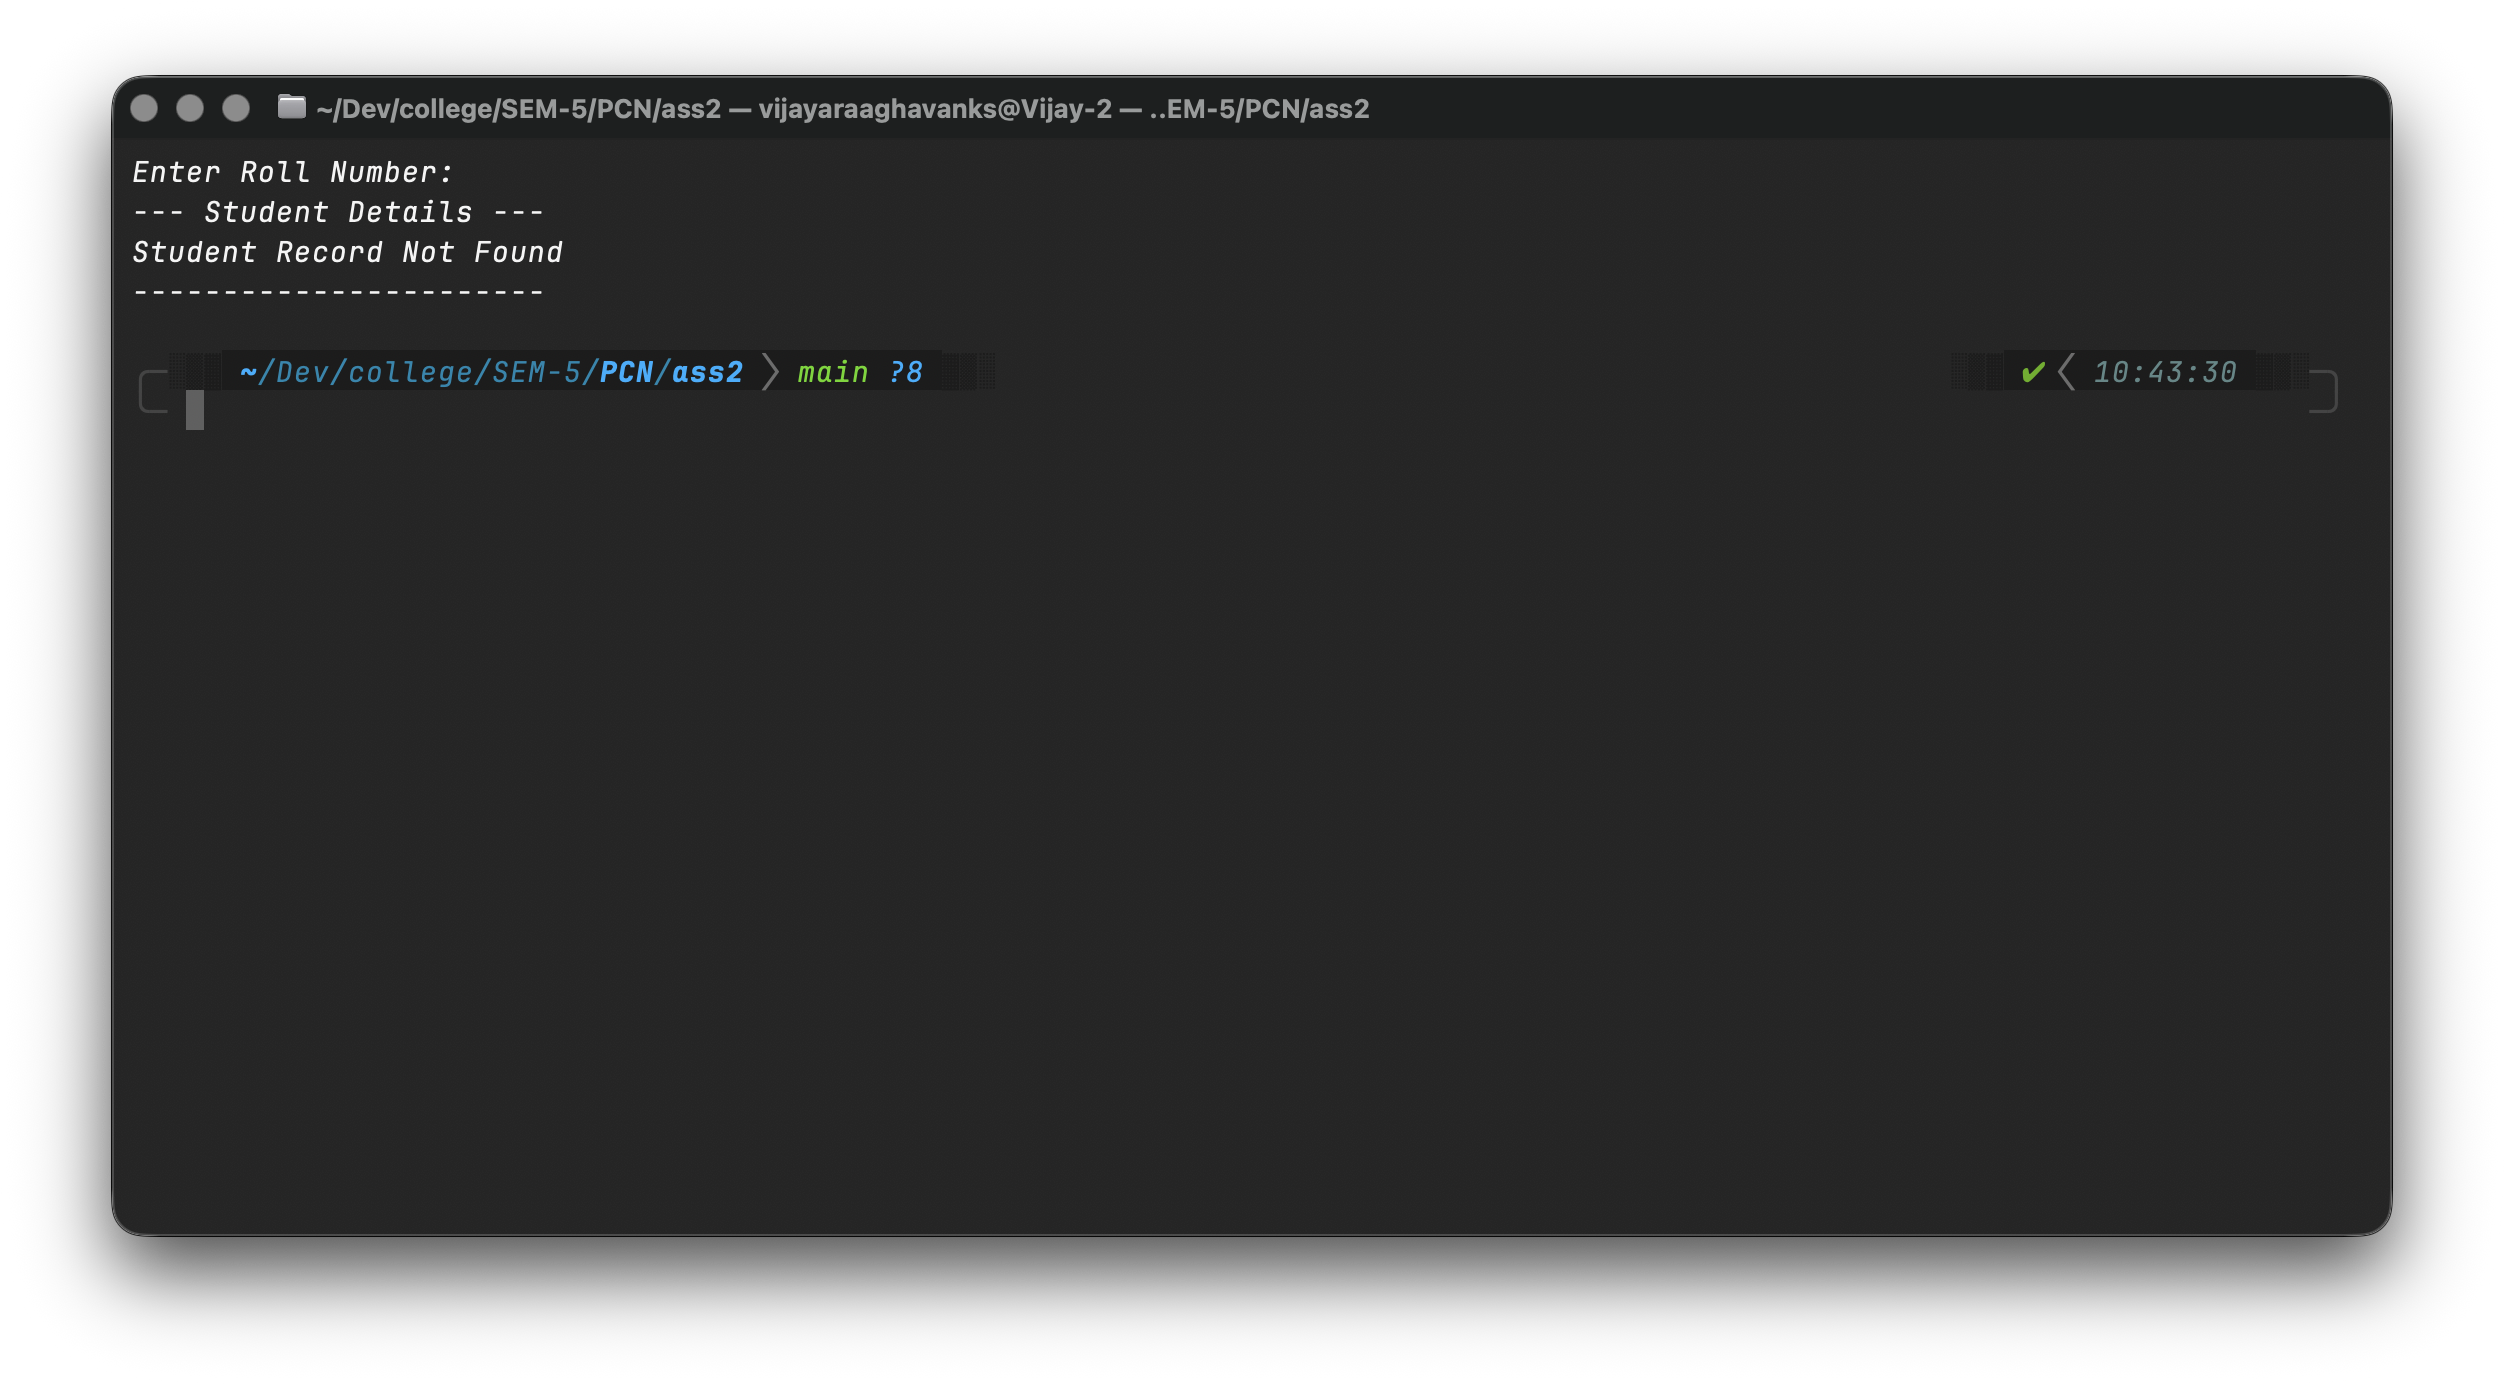
\includegraphics[width=0.62\linewidth]{screenshots/04_udp_client_notfound.png}
\caption{UDP client -- record not found (Roll Number 999)}
\end{figure}

\subsection*{6.2 Console Output (all test cases)}
\lstinputlisting[style=outstyle]{output.txt}

\section*{7. Comparison: TCP vs UDP}
\begin{center}
\renewcommand{\arraystretch}{1.3}
\begin{tabular}{p{2.6cm}p{5.6cm}p{5.6cm}}
\toprule
\textbf{Parameter} & \textbf{TCP (1a)} & \textbf{UDP (1b)} \\
\midrule
Connection & Connection-oriented; three-way handshake (\texttt{connect()}/\texttt{accept()}) sets up a dedicated channel. & Connectionless; each datagram is sent independently via \texttt{sendto()}. \\
Reliability & Reliable -- acknowledgments, timeouts and retransmission guarantee delivery. & Unreliable -- lost datagrams are silently dropped, no retransmission. \\
Ordering & Guaranteed in-order delivery via sequence numbers. & No ordering guarantee; datagrams may arrive out of order or be duplicated. \\
Error Recovery & Built-in checksum, duplicate/missing segment detection, flow \& congestion control. & Only a simple checksum; corrupted packets are dropped with no recovery. \\
Overhead & High -- 20-byte header, handshake and teardown packets, per-connection state. & Low -- 8-byte header, stateless, minimal overhead. \\
Concurrency & Concurrent server using one \texttt{pthread} per client. & Iterative single-threaded loop; stateless processing needs no threads. \\
\bottomrule
\end{tabular}
\end{center}

\section*{8. Learning Outcomes}
\begin{itemize}
  \item Understood how a TCP socket lifecycle (\texttt{socket}--\texttt{bind}--\texttt{listen}--\texttt{accept}) differs from the simpler UDP lifecycle (\texttt{socket}--\texttt{bind}--\texttt{recvfrom}/\texttt{sendto}).
  \item Learned to build a concurrent TCP server using POSIX threads so multiple clients can be served without blocking one another.
  \item Observed experimentally that TCP guarantees ordered, reliable delivery at the cost of connection-setup overhead, while UDP is lightweight but offers no delivery guarantee.
  \item Gained practical experience parsing a CSV-based record store and returning either full or partial records depending on protocol requirements.
  \item Understood why real-world protocols choose UDP for simple, latency-sensitive query/response exchanges and TCP for transfers that must be reliable and ordered.
\end{itemize}

\end{document}
